\section{Einleitung}
\label{sec:einleitung}

\paragraph{Motivation}
\begin{itemize}
  \item 50\% weniger Aufwand bei Anwendungsentwicklung mit DB
  \item Ermöglicht neue Anwendungen, die ohne DB zu komplex wären
  \item Ausfaktorisieren der Verwaltung großer Datenmengen
  \item \textbf{ohne Datenbanken}:
  \begin{itemize}
    \item Daten in Dateien abgelegt, Zugriffsfunktionalität Teil der Anwendung
    \item Redundanz (in Daten und Funktionalität)
    \item Programme oft nicht \emph{atomar} (= Programm wird entweder ganz oder gar nicht ausgeführt) --- nur bei nicht fehlerfreien Systemen relevant
    \item \emph{Transaktionen} (= Programm oder Kommandofolge) oft nicht \emph{isoliert} (= keine inkonsistenten Zwischenzustände sichtbar) --- nur bei mehreren Transaktionen, aber auch bei fehlerfreien Systemen relevant
    \item Nebenläufigkeit (\emph{concurrency} --- paralleler Zugriff auf dieselben Daten) schwer umsetzbar
    \item Anwendungsentwicklung abhängig von der physischen Repräsentation der Daten (z.B. Datenspeicherung als Tabelle: Reihenfolge Zeilen/Spalten muss bekannt sein)
    \item Datenschutz (kein unbefugter Zugriff) nicht gewährleistet
    \item Datensicherheit (kein Datenverlust, insb. bei Defekten) nicht gewährleistet
  \end{itemize}
\end{itemize}

\paragraph{Relationale Datenbanken}
\begin{itemize}
  \item auch \textbf{RDBMS} (\emph{relational database management system})
  \item[\( \cong \)] Menge von Tabellen
  \item Relation = Menge von Tupeln = Tabelle
\end{itemize}

\paragraph{RDBMS --- Terminologie}
\begin{itemize}
  \item \textbf{Relationenschema}: \emph{Fett} geschrieben
  \item \textbf{Relation}: Weitere Einträge der Tabelle
  \item \textbf{Tupel}: Eine Zeile der Tabelle
  \item \textbf{Attribut}: Spaltenüberschrift
  \item \textbf{Relationenname}: Name der Tabelle
  \item \textbf{DBS}: Datenbanksystem = DBMS + Datenbank(en)
  \item \textbf{Schlüssel}: Attribut, das nicht doppelt vergeben werden darf
  \item \textbf{Fremdschlüssel}: Attr taucht in anderem Relationenschema als Schlüssel auf
  \item \textbf{Integritätsbedingungen}:
  \begin{itemize}
    \item \emph{lokal}: Schlüssel in Relationenschema
    \item \emph{global}: Fremdschlüssel in Datenbankschema
  \end{itemize}
  \item \textbf{DB-Schema}: = Menge Relationsschemata + globale Integritätsbedingungen
  \item \textbf{Sicht} (\emph{view}): Häufig vorkommende Datenabfrage, kann mit Sichtnamen als "`virtuelle"' Tabelle gespeichert werden \\*
  \begin{lstlisting}[language=sql]
    create view CArtist as
      select NAME, JAHR
      from Kuenstler
      where LAND == "Kanada"
  \end{lstlisting}
  \item Verwendung wie "`normale"' Relation:
  \begin{lstlisting}[language=sql]
    select * from CArtist where JAHR < 2000
  \end{lstlisting}
  \item Nutzung für Datenschutz: Unterschiedliche Benutzer sehen unterschiedlichen DB-Ausschnitt
\end{itemize}

\paragraph{RDBMS --- Anfrageoperationen}
\begin{itemize}
  \item \textbf{Selektion}: Zeilen (Tupel) wählen (\( \sigma_{\text{KID}=1012}(\text{Titel}) \))
  \item \textbf{Projektion}: Spalten (Attribute) wählen (\( \pi_{\text{KID, NAME}}(\text{Kuenstler}) \))
  \item Beispiel komplexer Ausdruck: \( \pi_{\text{NAME}, \text{ART}}(\sigma_{\text{KID}=1012}(\text{Titel})) \)
  \begin{figure}[H]\centering\label{SelektionProjektion}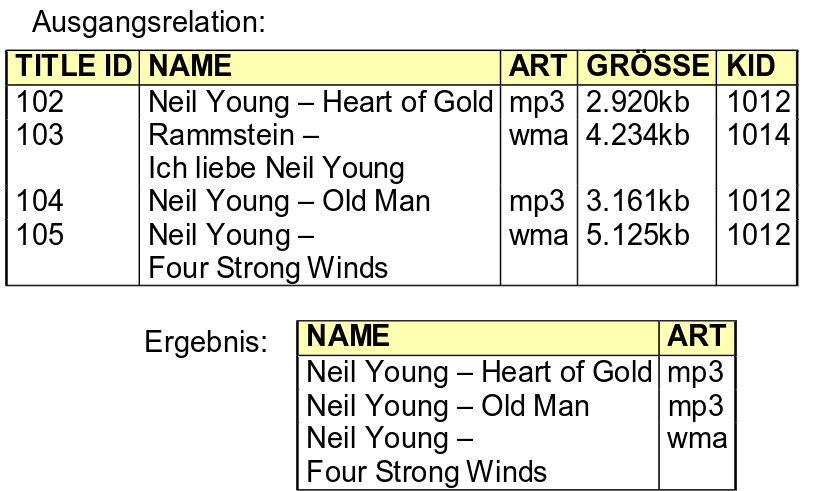
\includegraphics[width=0.3\textwidth]{SelektionProjektion}\end{figure}
  \item Weitere Operationen: Verbund (\emph{join}), Vereinigung, Differenz, Durchschnitt, Umbenennung
  \item Operationen beliebig kombinierbar (\( \leadsto \) Query-Algebra)
\end{itemize}

\paragraph{RDBMS --- Anfragenoptimierung}
Algebraische Ausdrücke äquivalent, Anfrage unterschiedlich komplex
\begin{itemize}
  \item \( \sigma_{\text{Vorname} = \text{'Klemens'}}(\sigma_{\text{Wohnort} = \text{'KA'}}(SNUSER)) \) vs.
  \item \( \sigma_{\text{Wohnort} = \text{'KA'}}(\sigma_{\text{Vorname} = \text{'Klemens'}}(SNUSER)) \)
\end{itemize}

\paragraph{RDBMS --- Physische Datenunabhängigkeit}
\begin{itemize}
  \item Anfragen \textbf{deklarativ}: Nutzer entscheidet nicht, wie Ergebnis ermittelt wird
  \item Datenunabhängigkeit: DBMS stellt sicher: \\*
    - stabile Anfragenfunktionalität bei physischer Darstellungsänderung \\*
    - Anfrage funktioniert bei unterschiedlichen Datenbanken (gleiches Schema, unterschiedliche Datenhäufigkeit)
  \item \( \leadsto \) erlaubt höhere Komplexität bei Anwendungsentwicklung
\end{itemize}

\paragraph{RDBMS --- 3-Ebenen-Architektur}
\begin{figure}[H]\centering\label{DreiEbenenSchema}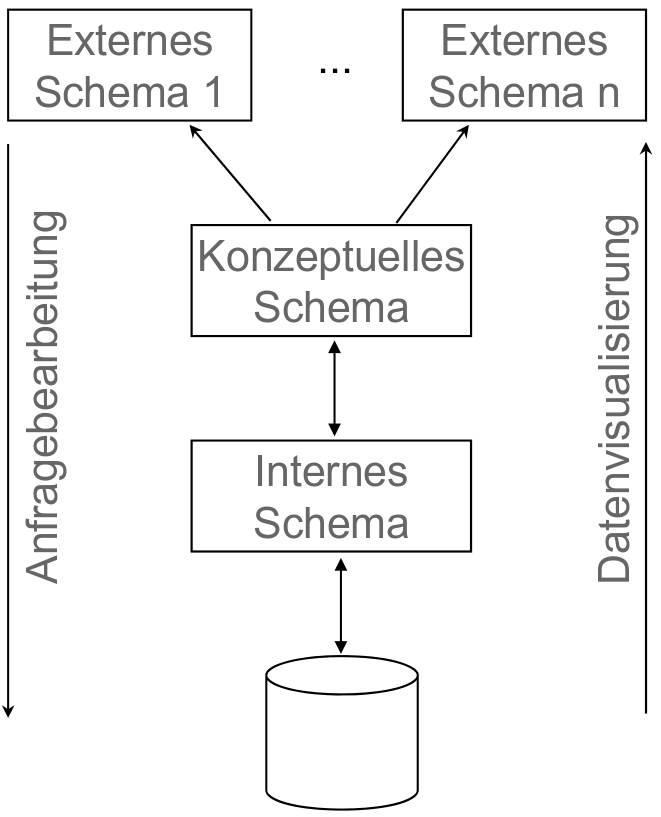
\includegraphics[width=0.15\textwidth]{DreiEbenenSchema}\end{figure}
\begin{itemize}
  \item \textbf{Konzeptionelles Schema}: Diskursbereich? Welche Entitäten interessant (bei Studierenden Noten interessant, Hobbies usw. nicht)?
  \item \textbf{Internes Schema}: physische Datenrepräsentation
  \item \textbf{Externe Schemata}: Unterschiedlicher Datenausschnitt für unterschiedliche Nutzer (Datenschutz, Übersichtlichkeit, organisatorische Gründe, Verstecken von Änderungen am konzeptionellen Schema)
  \item \( \leadsto \) \emph{Logische Datenunabhängigkeit}
\end{itemize}



\paragraph{Datenbankprinzipien --- Coddsche Regeln}
\begin{itemize}
  \item \textbf{Integration}: Einheitliche, nichtredundante Datenverwaltung
  \item \textbf{Operationen}: Speichern, Suchen, Ändern
  \item \textbf{Katalog}: Zugriff auf Datenbankbeschreibungen im data directory
  \item \textbf{Benutzersichten}
  \item \textbf{Integritätssicherung}: Korrektheit des DB-Inhalts
  \item \textbf{Datenschutz}: Ausschluss unauthorisierter Zugriffe
  \item \textbf{Transaktionen}: mehrere DB-Operationen als Funktionseinheit (= Atomarität)
  \item \textbf{Synchronisation}: parallele Transaktionen koordinieren (= Isolation)
  \item \textbf{Datensicherung}: Wiederherstellung von Daten nach Systemfehlern
  \item Strengste bekannte Datenbankdefinition
  \item Funktionale Anforderungen (nichtfunktional z.B.: Wie schnell/zuverlässig muss Dienst sein, kurze Antwortzeiten, Zuverlässigkeit, Effizienz, Skalierbarkeit)
\end{itemize}

\begin{fragen}
  \item Was ist eine Sicht?
  \item Was ist die relationale Algebra? Wozu braucht man sie?
  \item Geben Sie Beispiele für Algebra-Ausdrücke an, die nicht identisch, aber äquivalent sind, an.
  \item Was leistet der Anfragenoptimierer einer Datenbank?
  \item Erklären Sie: Drei-Ebenen-Architektur, physische/logische Datenunabhängigkeit.
\end{fragen}